\chapter{Project}

\section{Code Concept}

In extend to this article is a code base avaiable \footnote{\url{https://www.github.com/florianwiech/incremental-machine-learning}}.
This code base includes the reimplementation of EWC and the extension of modifying the Fisher Information Matrix.
The concept documents the code structure and procedure.

The complete code consists of three files.
"main.py", "network.py" and "mnist.py".

\begin{figure}[H]
    \centering
    
\includegraphics[scale=.4]{project/concept/files}
    \caption{File structure}
    \label{fig:concept_file_structure}
\end{figure}

The "\textbf{mnist.py}" makes the mnist dataset available.
It loads the mnist database automatically, reshapes the values and data structures and splits or permutes the dataset if neccesary.
After the calculation it returns the arrays in Python standard datastructures with the extension of multi-dimensional arrays from NumPy.
\newline
"\textbf{network.py}" holds the "Network" class.
The class consists of all neccesary operations for the EWC algorithm with original and adaption.
The contructor creates a neural network with 784 input neurons, three hidden layers with each 800 neurons and the ten mnist output classes.
In addition to that it initializes all neccesary functions like loss and accuracy.
After initialization the object offers several methods for training, testing and applying EWC to the task.
Figure \ref{fig:concept_class_diagram} shows a class diagram of the Network class.

\begin{figure}[H]
    \centering
    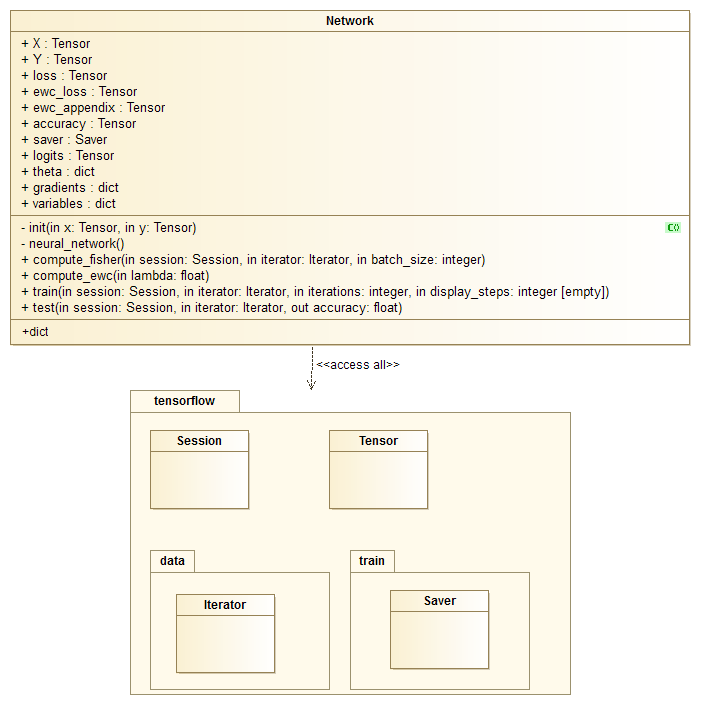
\includegraphics[scale=.6]{project/concept/class_diagram}
    \caption{Class diagram}
    \label{fig:concept_class_diagram}
\end{figure}

While execution the networks occupies multiple states.
The states distinguish if the network trains the first task or loads a previous state and retrains the network.
Figure \ref{fig:concept_state_diagram} shows the state diagram for the network:

\begin{figure}[H]
    \centering
    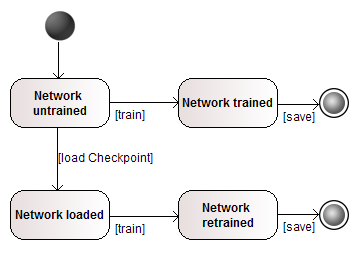
\includegraphics[scale=.8]{project/concept/state_diagram}
    \caption{State diagram}
    \label{fig:concept_state_diagram}
\end{figure}

"\textbf{main.py}" is the entrypoint of the code base.
It offers an command line tool for specification of the neccesary parameters.
\newline
The main function executes one tasks and saves their state in a checkpoint.
The task execution includes loading a checkpoint if it is not the first task or initialize a untrained network.
After that training or retraining the network and calculating the matrix if the new network should be saved.
Then perform an accuracy check on the testset and exit the script.
To train the second task the script has to be started again with different parameters.

The sequential execution is shown in a sequence diagram.
The first part (Figure \ref{fig:concept_sequence_diagram_part_1}) shows the initialization of all neccesary parameter and objects.
Part 2 (Figure \ref{fig:concept_sequence_diagram_part_2}) shows the execution of training and testing the neural network.

\begin{figure}[H]
    \centering
    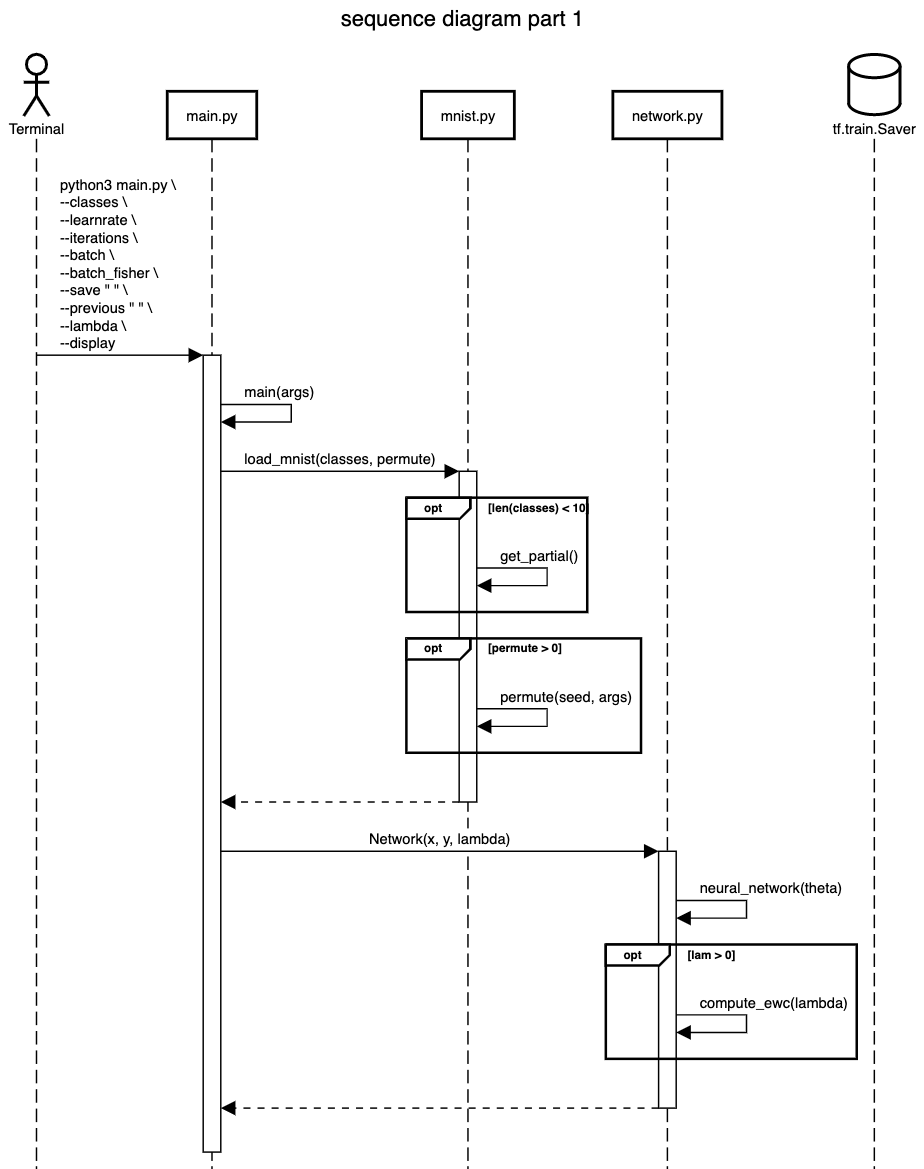
\includegraphics[width=\textwidth]{project/concept/sequence_diagram_part_1}
    \caption{Sequence diagram part 1}
    \label{fig:concept_sequence_diagram_part_1}
\end{figure}

\begin{figure}[H]
    \centering
    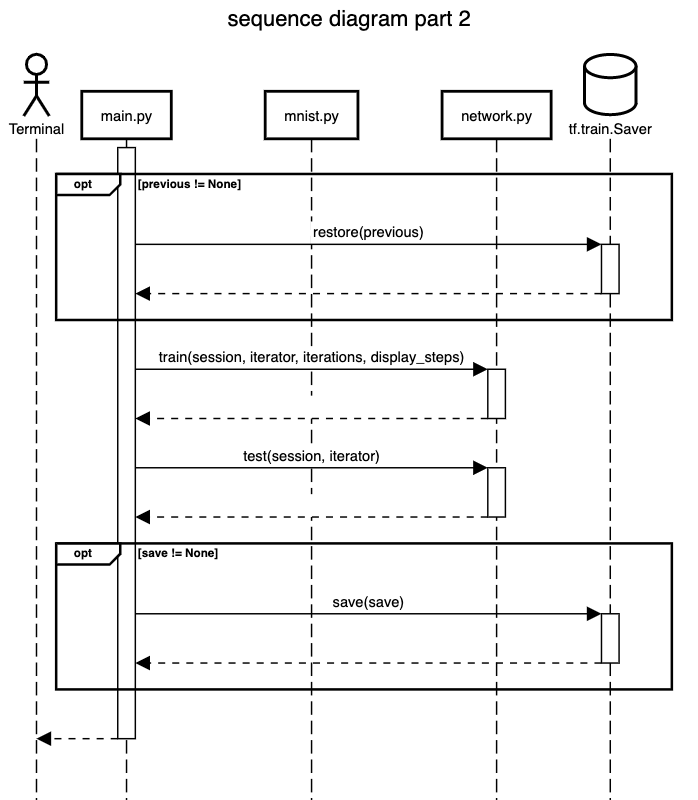
\includegraphics[width=\textwidth]{project/concept/sequence_diagram_part_2}
    \caption{Sequence diagram part 2}
    \label{fig:concept_sequence_diagram_part_2}
\end{figure}

\section{Theory}
\newpage
\section{Baseline}

Before adapting the EWC algorithm the codebase has to proof, that it delivers the results of the EWC paper.
The original EWC algorithm was tested in the constructed benchmarks described in Project Goals (Section \ref{project_goals}):

\subsection{Disjoint 9-1 benchmark}

$T_1$ (blue, $\bigtriangleup$) trained with the classes zero to eight and reaches an accuracy of 95.72\% at the end of its training pahse.
The task was trained with a learnrate of 0.001, 2500 iterations and an batch size of 100.
In comparison to the complete dataset (green, line), the accuracy is 86.06\%.

$T_2$ (yellow, $\bullet$) trained with the class nine further of $T_1$ uses a learnrate of 0.00001, 2500 iterations and a batch size of 100.
The lambda value is $\frac{1}{learnrate = 0.00001} = 100,000$.
It reaches an accuracy of 97.81\%.

At the end of $T_2$ trainng phase designates $T_1$ to 84.50\% and the complete dataset 85.44\%.
The complete dataset reaches a peak of 93.43\% where $T_1$ has 94.87\% precision and $T_2$ 76.66\% precision.

Figure \ref{fig:ewc_d9-1} shows the trainings of both tasks compared to the accuracy of the complete dataset:

\begin{figure}[H]
    \centering
    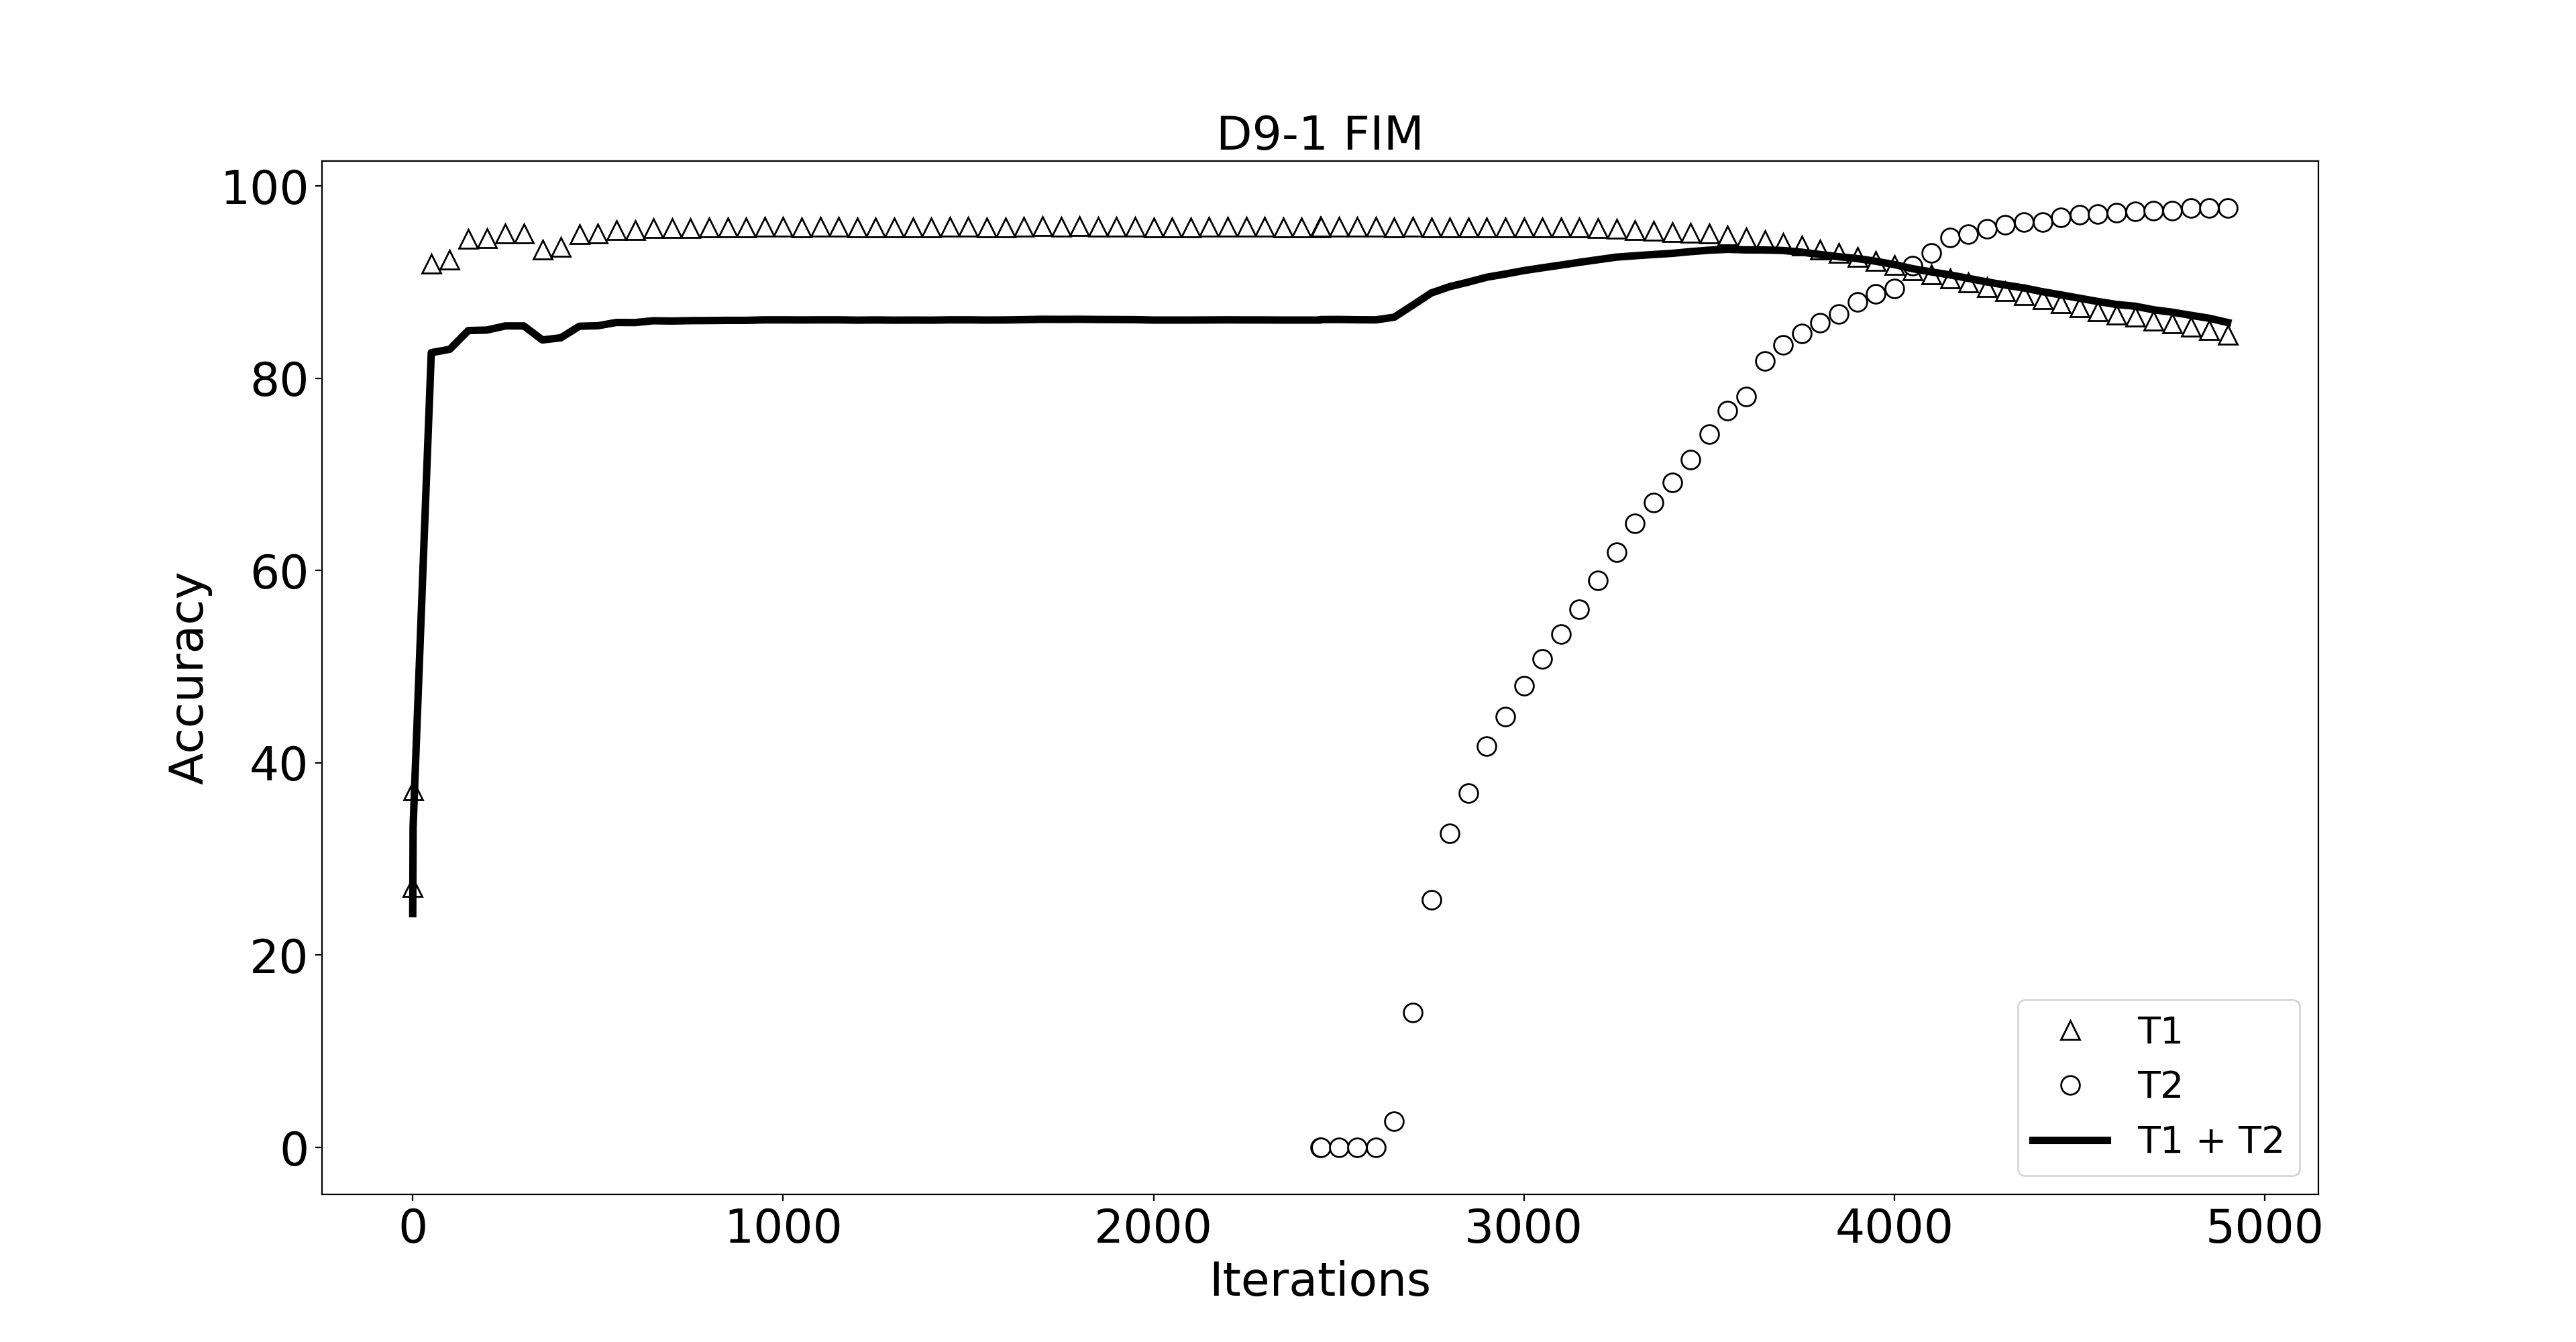
\includegraphics[width=\textwidth]{project/baseline/D91_FIM}
    \caption{EWC D9-1}
    \label{fig:ewc_d9-1}
\end{figure}

\subsection{Disjoint 5-5 benchmark}

Figure \ref{fig:ewc_d5-5} shows training of a disjoint mnist with a five class split.

The first Task $T_1$ (blue, $\bigtriangleup$) with the classes zero to four, reached an accuracy of 98.66\% after the first training.
$T_1$ is trained with a learnrate of 0.001, 2500 iterations and a batch size of 100.
Since there are only five of ten possible classes trained, the accuracy on the complete dataset amounts 50.70\%.

In the second training phase with task $T_2$ (yellow, $\bullet$), the classes five to nine achieve an accuracy of 82.67\%.
The learnrate of $T_2$ is 0.00001 and there were again 2500 iterations and a batch size of 100.
Since it is an ongoing task, the EWC appendix is applied to the loss.
In this case lambda was set to $\frac{1}{learnrate = 0.00001} = 100,000$.

After the second training had $T_1$ lost 22.22\%, but still shows a quality of 76.44\%.
The performance of the complete dataset ascended from 50.70\% to 79.39\%.

\begin{figure}[H]
    \centering
    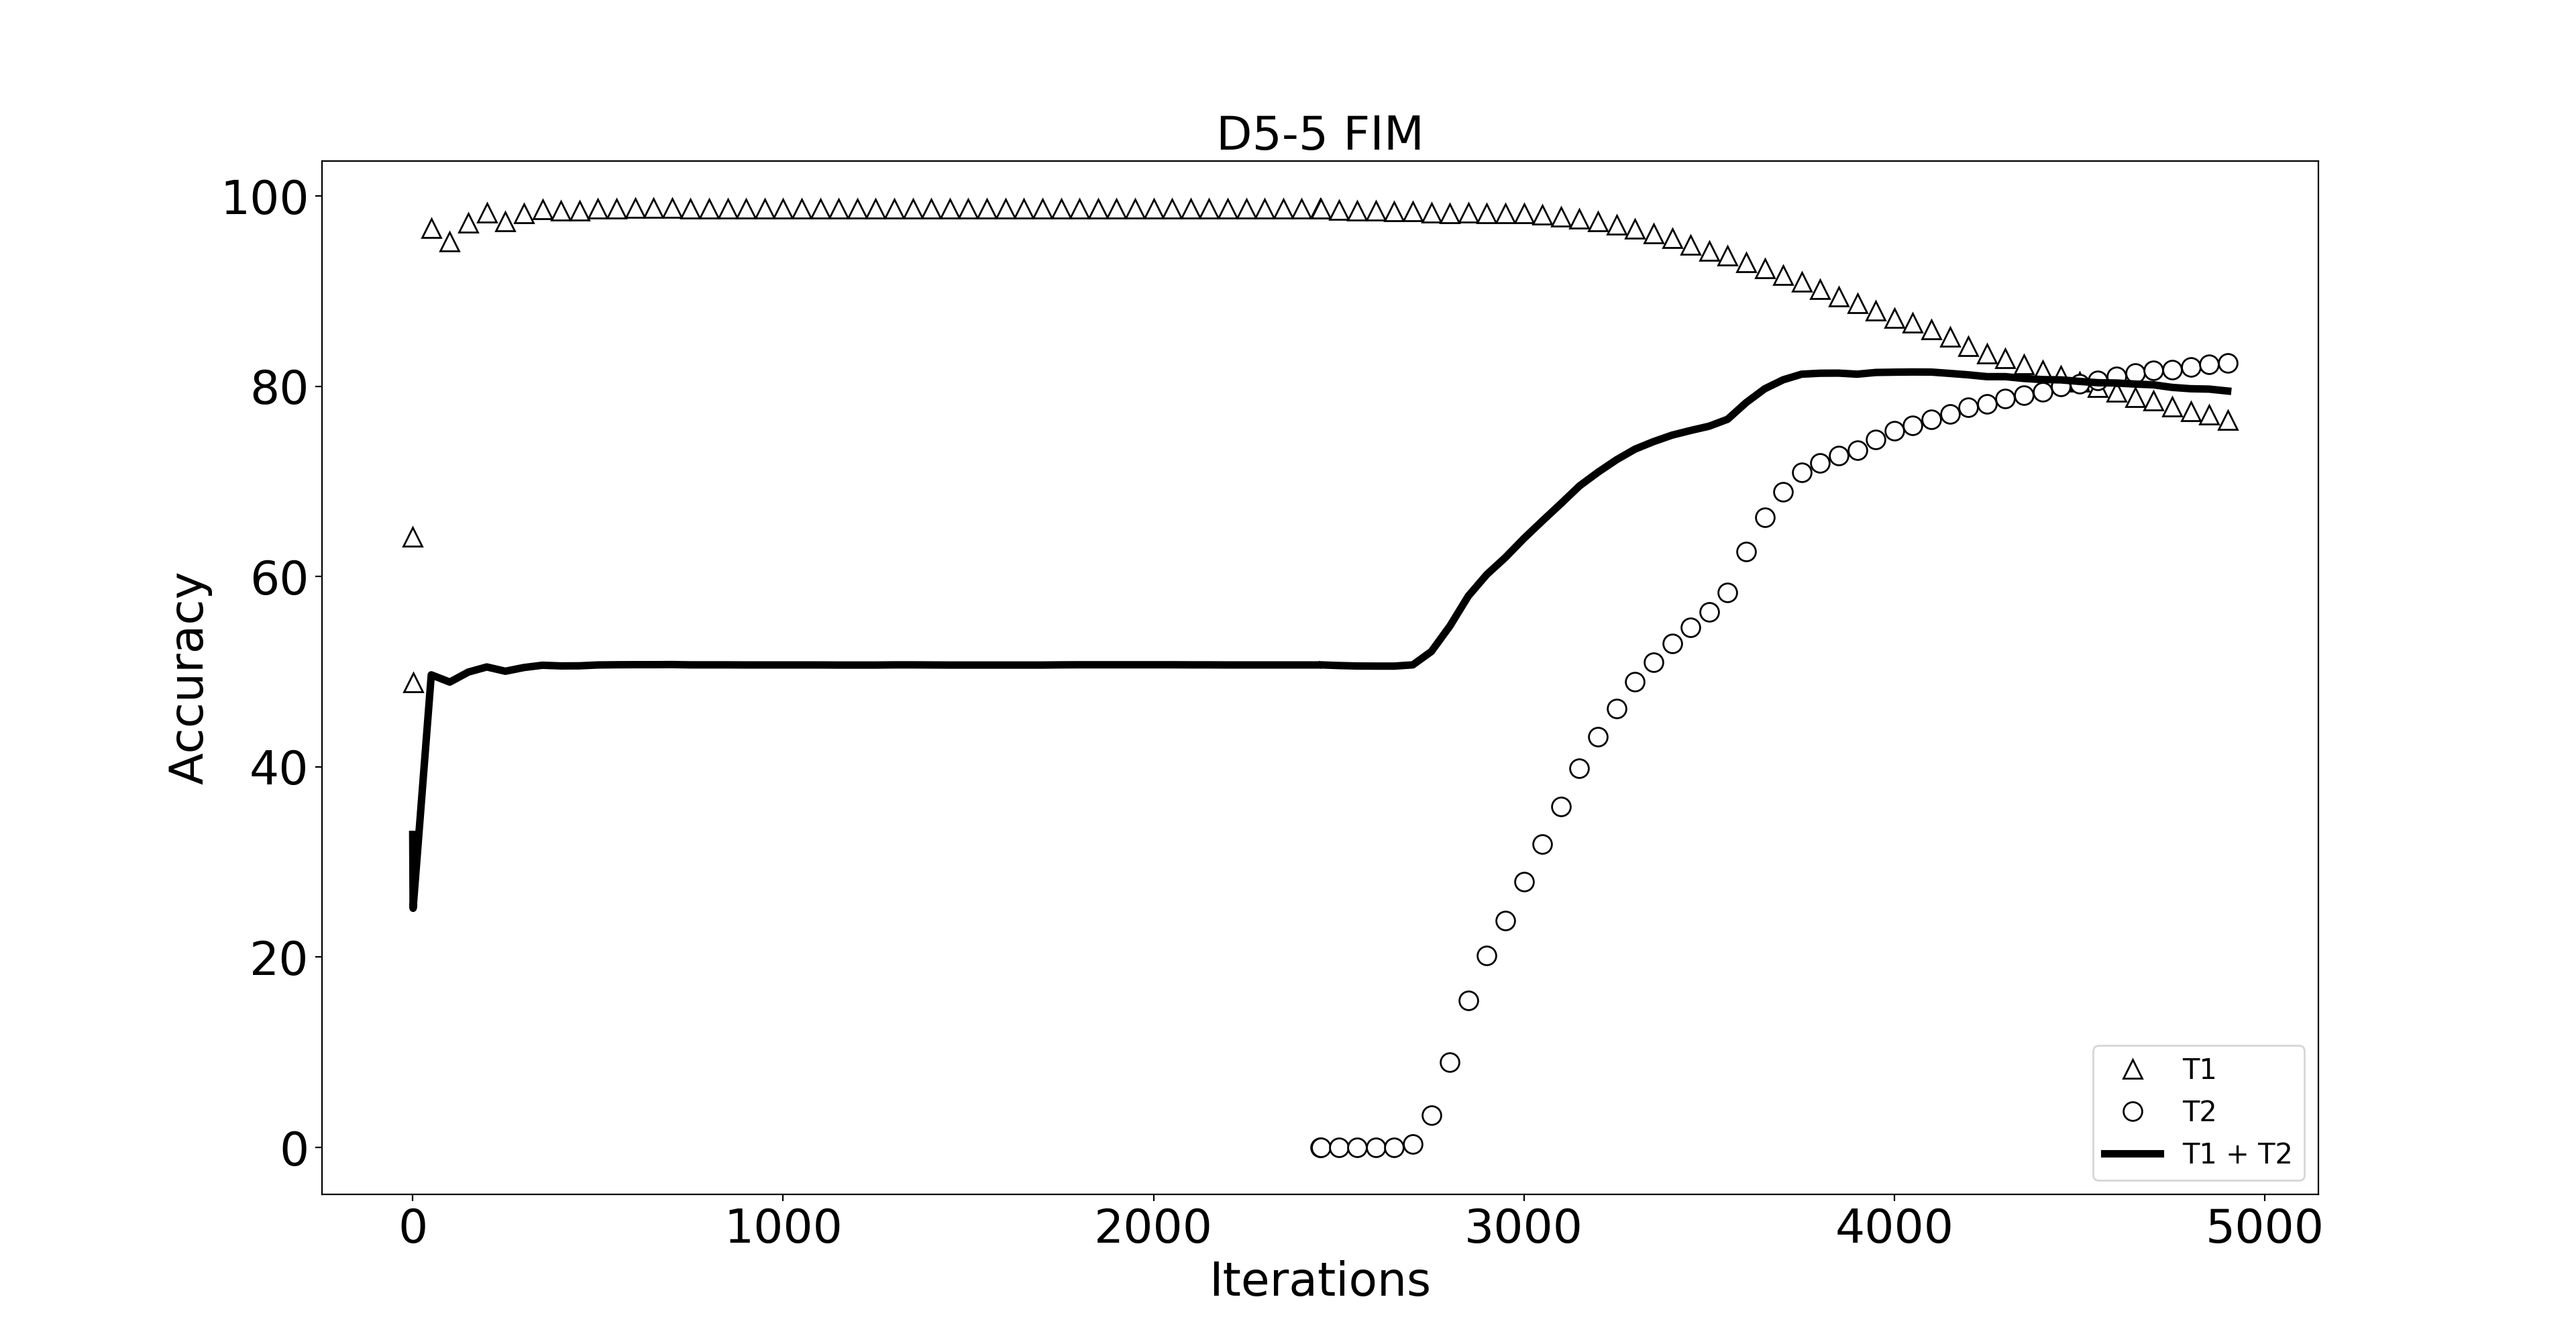
\includegraphics[width=\textwidth]{project/baseline/D55_FIM}
    \caption{EWC D5-5}
    \label{fig:ewc_d5-5}
\end{figure}

\subsection*{Permuted 10-10 benchmark}

EWC performance is shown in Figure \ref{fig:ewc_p10-10}.
$T_1$ is trained with following parameters:
all classes with a
learnrate of 0.001,
60,000 samples,
batch size of 100 in
2500 iterations.
After the $T_1$ training, it shows an accuracy of 94.76\% which is equally to the complete dataset.
\newline
$T_2$ on the other hand learned with a rate of 0.00001 with 20,000 iterations.
The 60,000 samples were permuted with a seed of zero and split into batches with a size of 100.
The importance of the EWC loss was $\lambda = \frac{1}{0.00001} = 100,000$.
$T_2$ needed in this case a longer learnrate to be able to have an good accuracy.
It shows a performance of 91.45\% and 90.53\% on the complete dataset.
$T_1$ still performs with 94.78\%.

\begin{figure}[H]
    \centering
    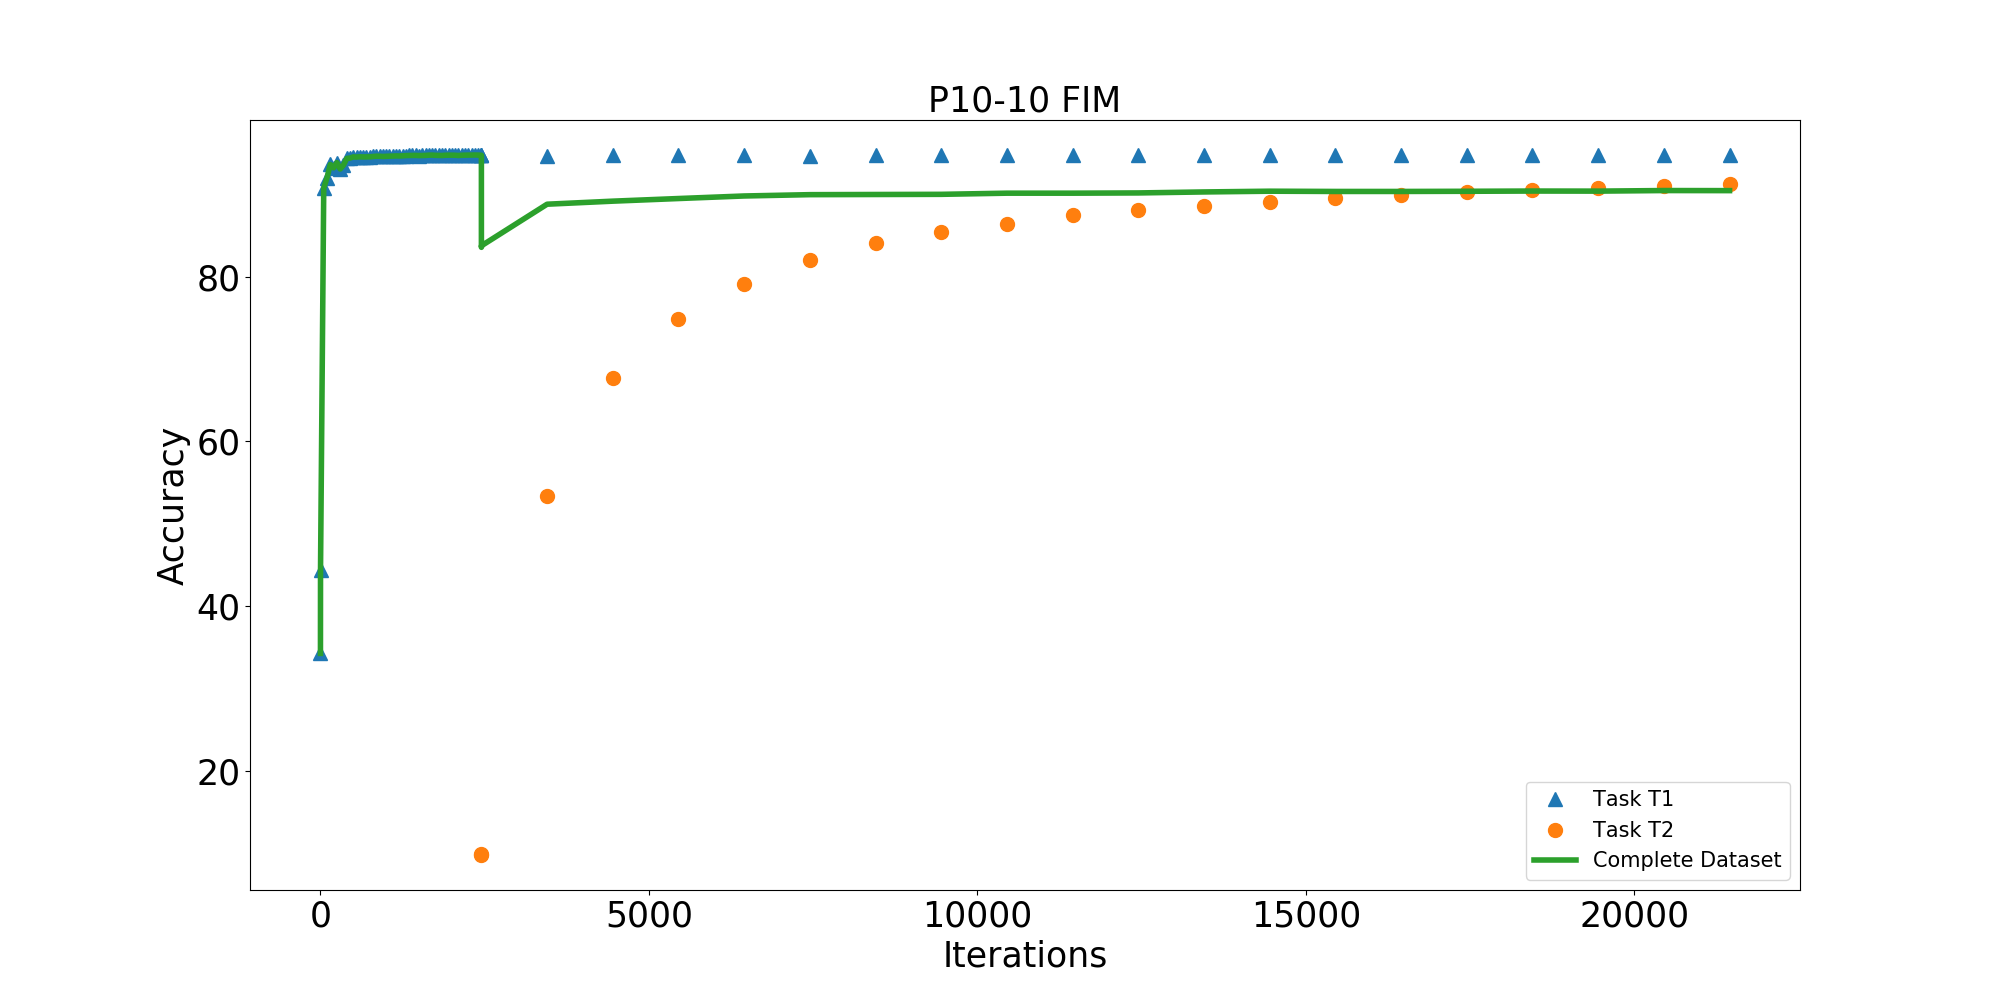
\includegraphics[width=\textwidth]{project/baseline/P10-10_FIM_IT20k}
    \caption{EWC P10-10}
    \label{fig:ewc_p10-10}
\end{figure}


Figure \ref{fig:ewc_d9-1} shows the trainings of both tasks compared to the accuracy of the complete dataset:

\begin{figure}[H]
    \centering
    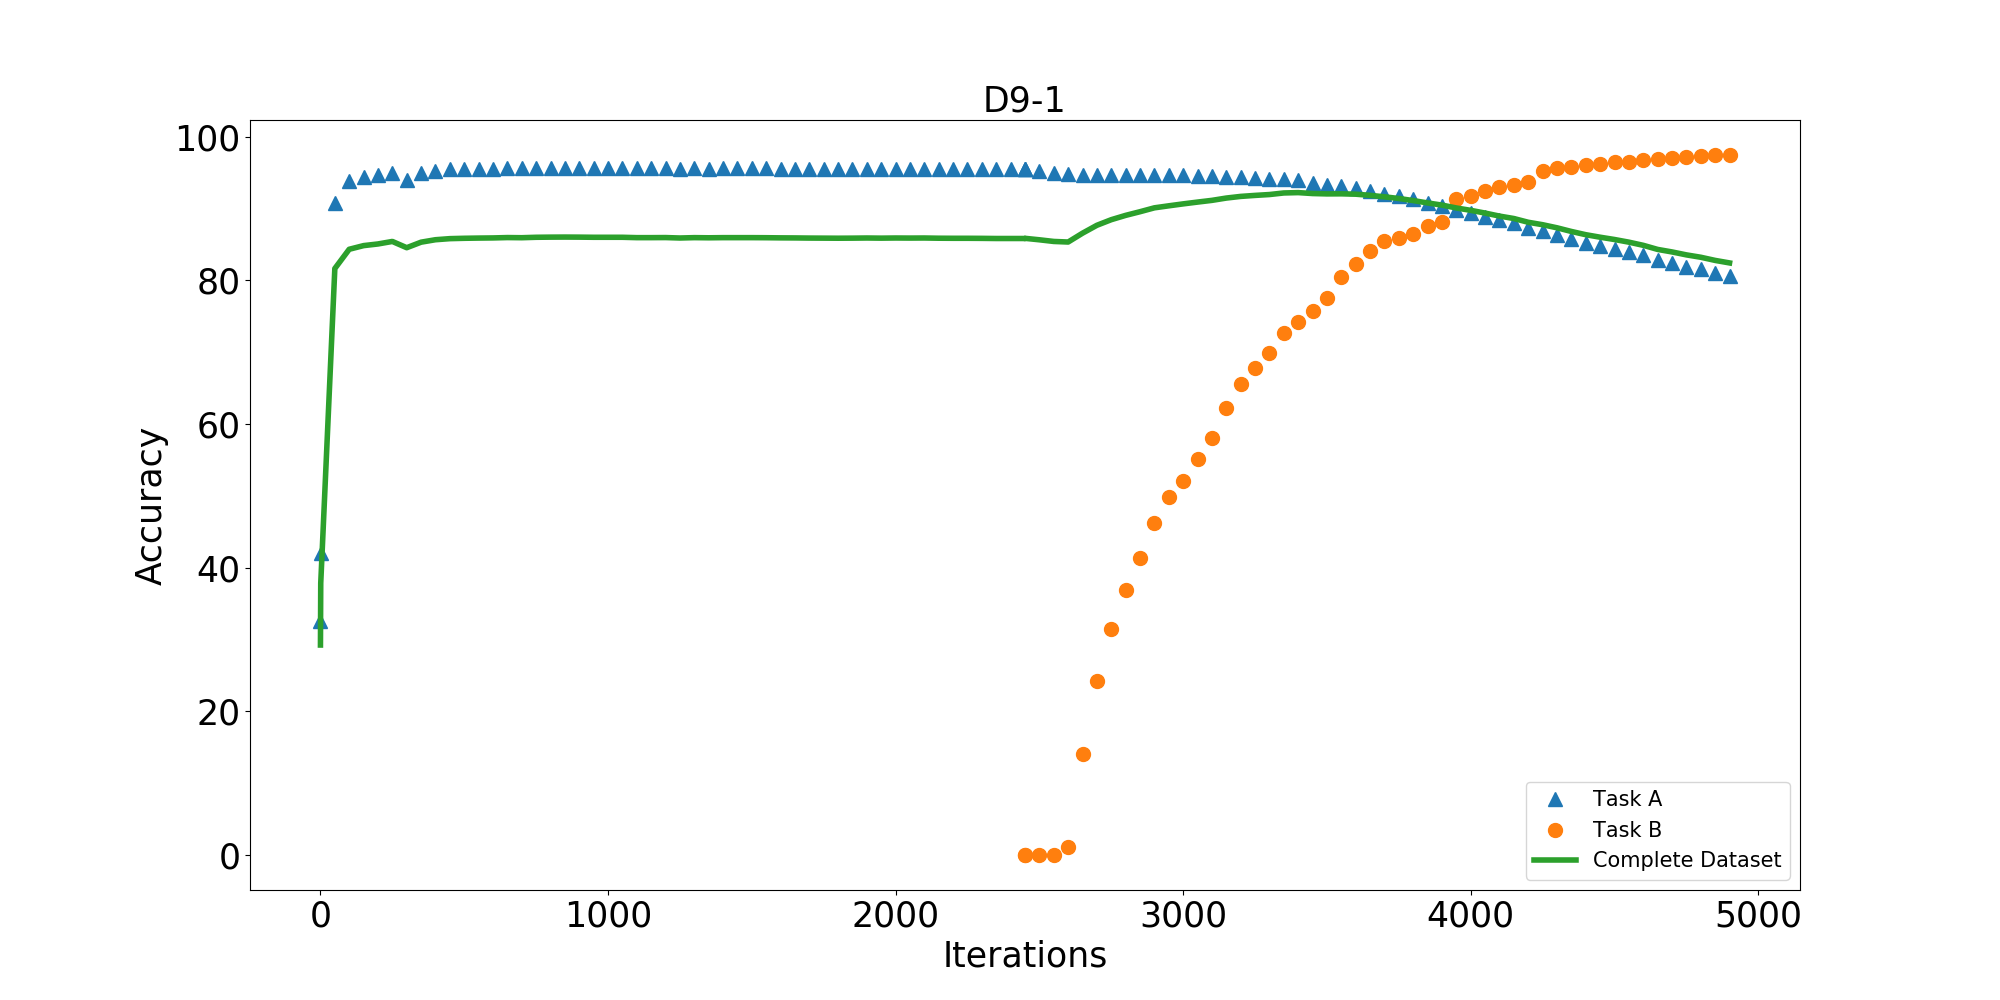
\includegraphics[width=\textwidth]{project/baseline/D9-1_BS1}
    \caption{EWC D9-1}
    \label{fig:ewc_d9-1}
\end{figure}

\subsection*{Permuted 10-10 benchmark}



\begin{figure}[H]
    \centering
    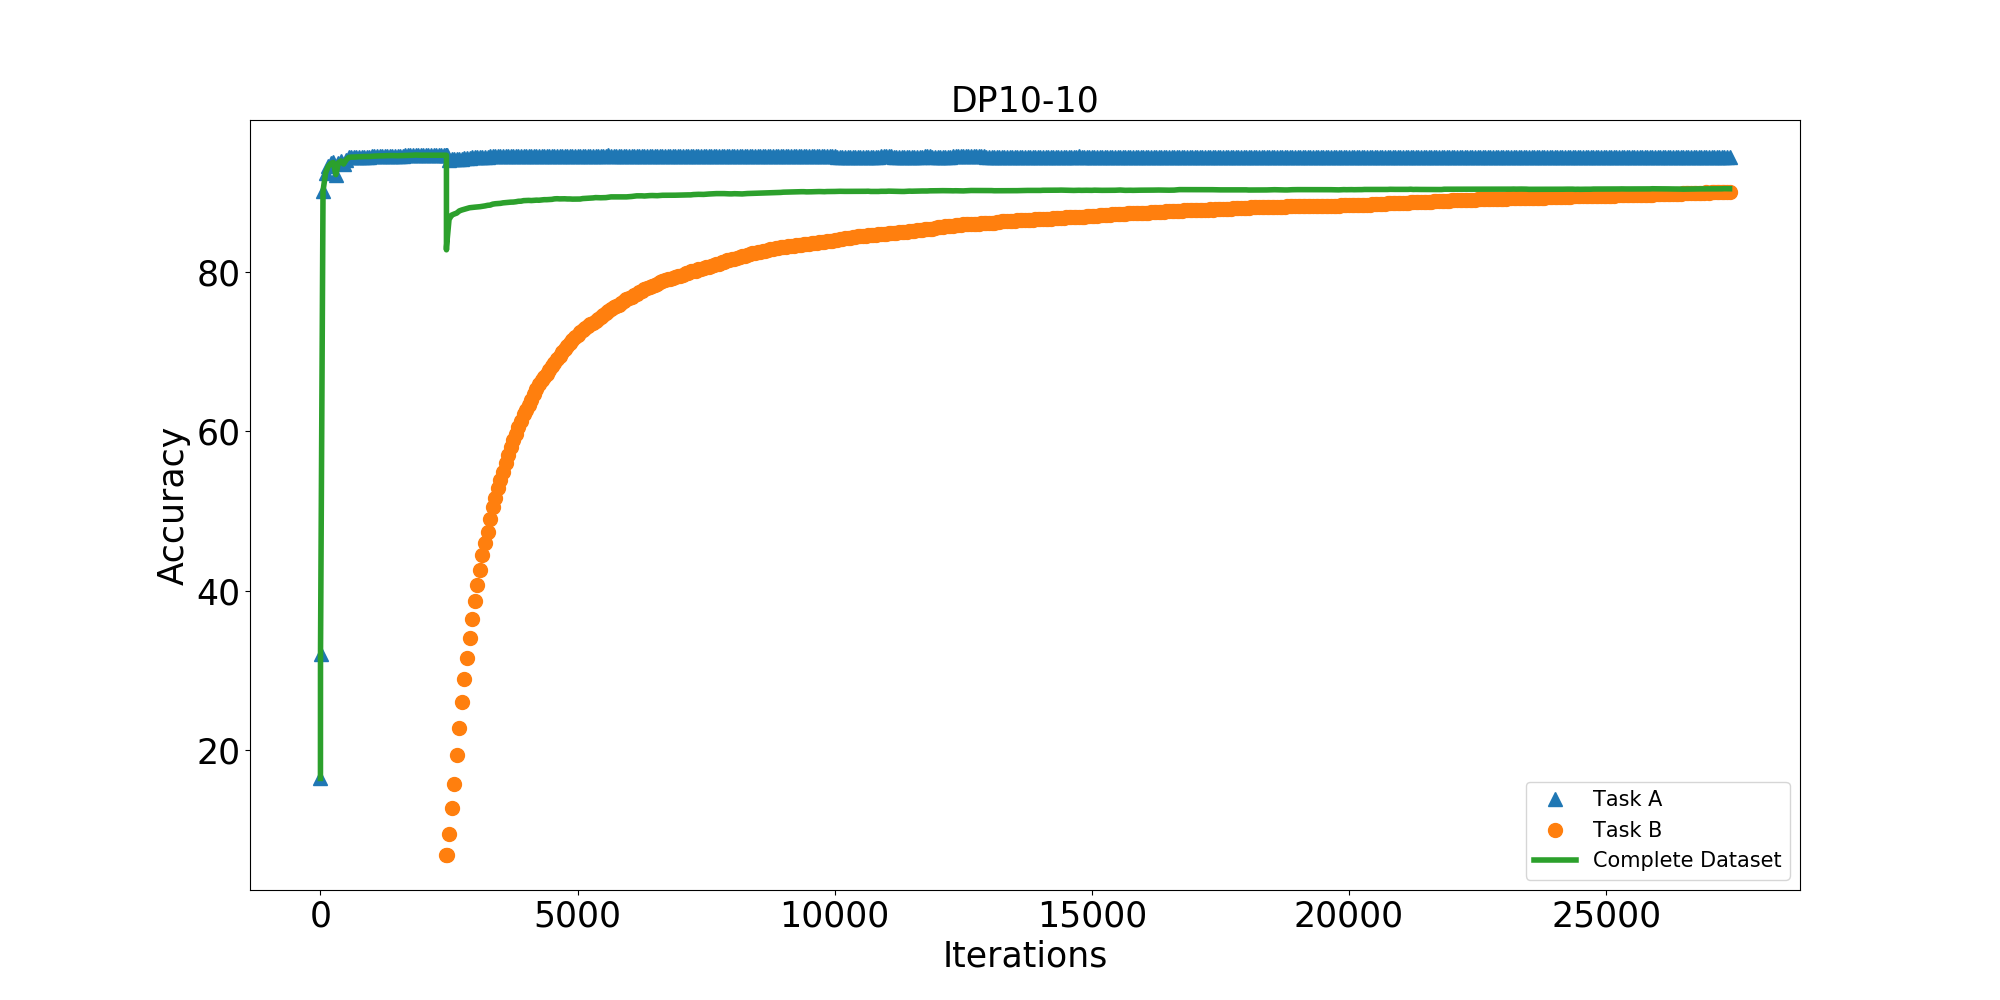
\includegraphics[width=\textwidth]{project/baseline/P10-10_BS1}
    \caption{EWC P10-10}
    \label{fig:ewc_p10-10}
\end{figure}

\section{Experiments}

